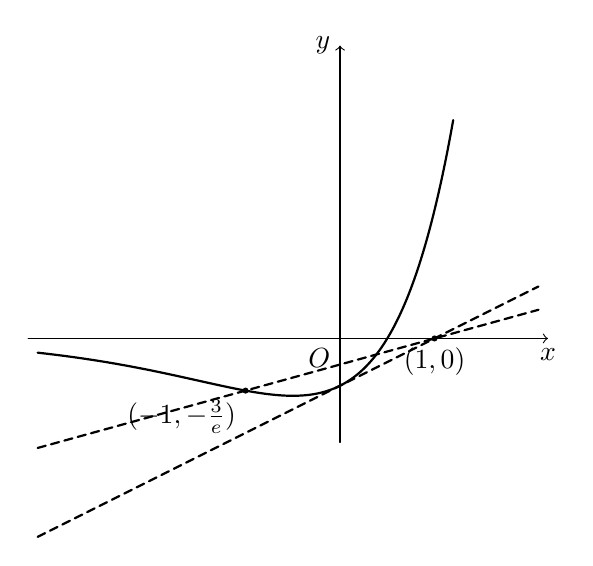
\begin{tikzpicture}[x=1.2cm,y=0.6cm,line cap=round,line join=round]
  \draw[->] (-3.3,0) -- (2.2,0) node[below] {$x$};
  \draw[->] (0,-2.2) -- (0,6.2) node[left] {$y$};
  \node[below left] at (0,0) {$O$};

  % 曲线 y=e^x(2x-1)
  \draw[thick,smooth,samples=220,domain=-3.2:1.2]
    plot (\x,{exp(\x)*(2*\x-1)});

  % 第一条虚线：y=x-1（题图里那条“切线”示意）
  \draw[densely dashed,thick] (-3.2,{-3.2-1}) -- (2.1,{2.1-1});

  % 点 (-1,-3/e) 与 (1,0)
  \pgfmathsetmacro{\yB}{-3/exp(1)} % -3/e
  \fill (-1,\yB) circle (1.1pt);
  \node[below left] at (-1,\yB) {$(-1,-\frac{3}{e})$};

  \fill (1,0) circle (1.1pt);
  \node[below] at (1,0) {$(1,0)$};

  % 第二条虚线：过 (1,0) 与 (-1,-3/e)
  % 斜率 m = (0-(-3/e))/(1-(-1)) = 3/(2e)
  % 方程 y = (3/(2e))(x-1)
  \pgfmathsetmacro{\m}{3/(2*exp(1))}
  \draw[densely dashed,thick]
    (-3.2,{\m*(-3.2-1)}) -- (2.1,{\m*(2.1-1)});
\end{tikzpicture}